\documentclass[letter,10pt]{article}

\usepackage{amsmath, amsxtra, amsfonts,amscd,amssymb}
\usepackage{algorithm,algorithmic}
\usepackage{graphicx}
\usepackage{epstopdf}
\usepackage{url}
\usepackage[left=1in,top=1in,right=1in,bottom=1in,letterpaper]{geometry}
\usepackage{setspace}
\usepackage{listings}
\usepackage{color}
\definecolor{mygreen}{RGB}{28,172,0} % color values Red, Green, Blue
\definecolor{mylilas}{RGB}{170,55,241}
\onehalfspace

\title{Data reconstruction based on incomplete inter- point distance}
\author{Name: Yunyun Zhang, Yiheng Chen  \\
             RIN : 661482565, 661482522
           }
\date{}

\begin{document}

\lstset{language=Matlab,%
    %basicstyle=\color{red},
    breaklines=true,%
    morekeywords={matlab2tikz},
    keywordstyle=\color{blue},%
    morekeywords=[2]{1}, keywordstyle=[2]{\color{black}},
    identifierstyle=\color{black},%
    stringstyle=\color{mylilas},
    commentstyle=\color{mygreen},%
    showstringspaces=false,%without this there will be a symbol in the places where there is a space
    numbers=left,%
    numberstyle={\tiny \color{black}},% size of the numbers
    numbersep=9pt, % this defines how far the numbers are from the text
    emph=[1]{for,end,break},emphstyle=[1]\color{red}, %some words to emphasise
    %emph=[2]{word1,word2}, emphstyle=[2]{style},    
}

\maketitle
\abstract{The main topic is data reconstruction based on incomplete inter-point distance. In this project, given less than 4 percentage of the total original data which contains the distance between any two points on the surface of a 3D object, then recover the complete matrix from the given data using the low-rank matrix completion theory. To complete the goal, singular value thresholding (SVT) algorithm is used in this project. This paper is an explanation of the algorithm as well as the results.}

\section{Problems}
Consider a set of points $\{x_1, ..., x_n\}$ sampled on a surface $\mathcal{M}\in\mathbb{R}^3.$ Given
small portion of the distance matrix $||x_i-x_k||_2, (i, j)\in\Omega$. Reconstruct $\{x_1, ..., x_n\}$ using the low-rank matrix completion theory.

\textbf{Contributions:}

We discuss and write the approaches for the problem together. Then each of us writes one half of the report. Yunyun Zhang writes section Abstract and Methodology.
Yiheng Chen writes section Problem, Results, and Observation.

\section{Methodology}
\label{sec:method}
\subsection{Model}
We want to find the lowest rank matrix $X$ which matches the matrix $M$, for all entries in the set $\Omega$ of given entries. The mathematical formulation can be written as follows:
\begin{equation}
\label{eqn:model1}
\min_{x} \text{rank}(X) \quad \text{s.t.} \quad X_{ij} = M_{ij} \quad \forall i, j\in \Omega
\end{equation}

Since the problem is NP-hard, we introduce another optimization problem to solve the matrix completion.
As \cite{cai2008} states, most of matrices $M$ can be exactly reconstructed by solving the optimization problem
\begin{equation}
\min_{x} ||X||_* \quad \text{s.t.} \quad X_{ij} = M_{ij} \quad \forall i, j\in \Omega
\end{equation}
where $||X||_*$ is the nuclear norm of the matrix $M$.

\subsection{The Singular Value Thresholding Algorithm}

\subsubsection{The singular value shrinkage operator}
Consider the Singular Value Decomposition of matrix $X$,
\begin{equation}
X=\mathbf{U\Sigma V^*}, \quad \mathbf{\Sigma}=\text{diag}(\{\sigma_i\}_{1<i<r})
\end{equation}
where $\mathbf{U}$ and $\mathbf{V}$ are orthogonal matrices.

For each $\tau \geq 0$, we define the soft-thresholding operator $\mathcal{D}_\tau$:

\begin{equation}
\mathcal{D}_\tau(X):=\textbf{U}\mathcal{D}_\tau(\Sigma)V^*, \quad \mathcal{D}_\tau(\Sigma)=
\text{diag}(\{\sigma_i-\tau_+\})
\end{equation}

where $\tau_+=\text{max}(0,t)$. According to the proof in \cite{cai2008}, the above equation is equivalent to:

\begin{equation}
\mathcal{D}_\tau(Y)=\arg\min_{X} \frac{1}{2}||X-Y||_F^2+\tau||X||_*
\end{equation}

\subsubsection{Shrinkage iterations}

For a fixed $\tau > 0$, a sequence $\{\delta_k\} \geq 0$ of step sizes and $k=1, 2, ...,$
\[
\begin{cases}
X^k=\mathcal{D}_\tau(Y^{k-1}),\\
Y^k=Y^{k-1}+\delta_k\mathcal{P}_\Omega(M-X^k)
\end{cases}
\]

Starting with $Y_0$ until a stopping criterion is reached.

\subsubsection{Stopping criteria}

As \cite{cai2008} proved, the sequence $\{X^k\}$ converges to the unique solution of an minimization problem:

\begin{equation}
\min_{x} \tau||X||_*+\frac{1}{2}||X||_F^2 \quad \text{s.t.} \quad X_{ij} = M_{ij} \quad \forall i, j\in \Omega
\end{equation}

which is closely related to equation (2).
The stopping criterion is motivated by the first-order optimality conditions or KKT conditions
tailored to the equation (6). The solution to the equation (6) must satisfy following two condition.

\[
\begin{cases} 
X=\mathcal{D}_\tau(Y),\\
\mathcal{P}_\Omega(X-M) = 0 
\end{cases}
\]
where Y is a matrix vanishing outside of $\Omega^c$. By definition, the first equation is always be true. Then the stopping criteria equation defined as second equation is less than a predefined tolerance.

\begin{equation}
\frac{||\mathcal{P}_\Omega(X^k-M)||_F}{||\mathcal{P}_\Omega(M)||_F} \leq \epsilon
\end{equation}

where $\epsilon$ is a fixed tolerance, and we set $\epsilon = 0.015$ in the project. 

\subsubsection{Choose value}

\noindent We use step size $\delta=1.2 \text{ times the undersampling ratio}$ from \cite{cai2008}.

\noindent Parameter $\tau=3000$ and increment $l=5$ are chosen empirically.

\subsubsection{Algorithm}
\begin{algorithm}[H]
\caption{Singular Value Thresholding algorithm}
\begin{algorithmic}
\STATE{\textbf{Step 0.}} Initialize $\delta, \tau, l$

\qquad\qquad Initialize $Y_0 = 0$

 \WHILE{not converge}
 
\STATE{\textbf{Step 1.}} Updating formula for $X$.

\qquad\qquad $X_k=\mathcal{D}_\tau(Y^{k-1})$

\STATE{\textbf{Step 2.}} Updating formula for $Y$.

\qquad\qquad $Y_k=Y_{k-1}+\delta_k\mathcal{P}_\Omega(M-X^k)$

\ENDWHILE


\end{algorithmic}
\end{algorithm}


\section{Results}

The recovery is performed via the SVT algorithm , and we use
\begin{equation}
\frac{||\mathcal{P}_\Omega(X^k-M)||_F}{||\mathcal{P}_\Omega(M)||_F} \leq 0.015
\end{equation}
as a stopping criterion. During the process, we choose the step sizes are constant and we set $\delta = 1.2*n*n/m $. The size of full unknown distance matrix is 401231*401231, and the given distance matrix size is 2601*2601. 
The relative error defined as 
\begin{equation}
\frac{||(X^{opt}-M)||_F}{||(M)||_F} 
\end{equation}
The computational result is shown within 200 iteration, the iteration error is smaller than 0.015. 

\begin{figure}[H]
\centering
\begin{minipage}{0.495\linewidth}
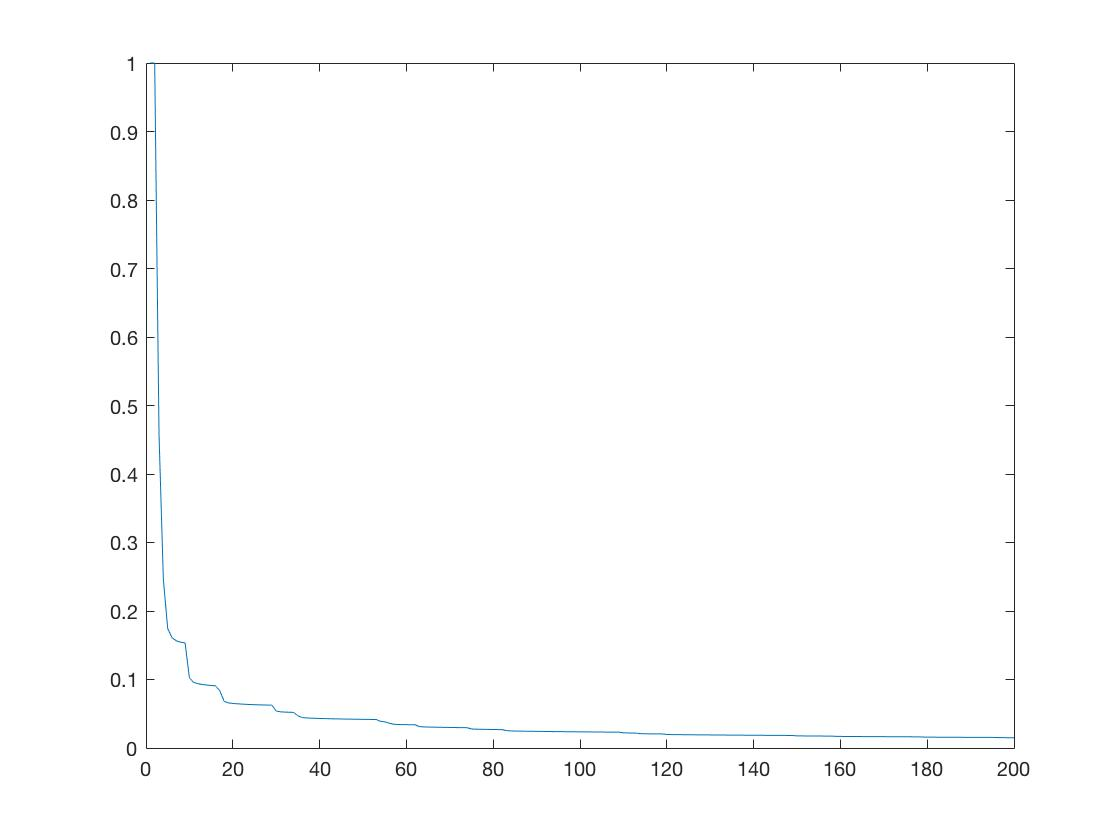
\includegraphics[width=1\linewidth]{error.jpg}\\
\end{minipage}\hfill
\caption{Relative error}
\end{figure}

The running time is approximate 5 minutes on my computer, but the running may varies, since it depends on the configuration of the laptop.

\begin{figure}[H]
\centering
\begin{minipage}{0.495\linewidth}
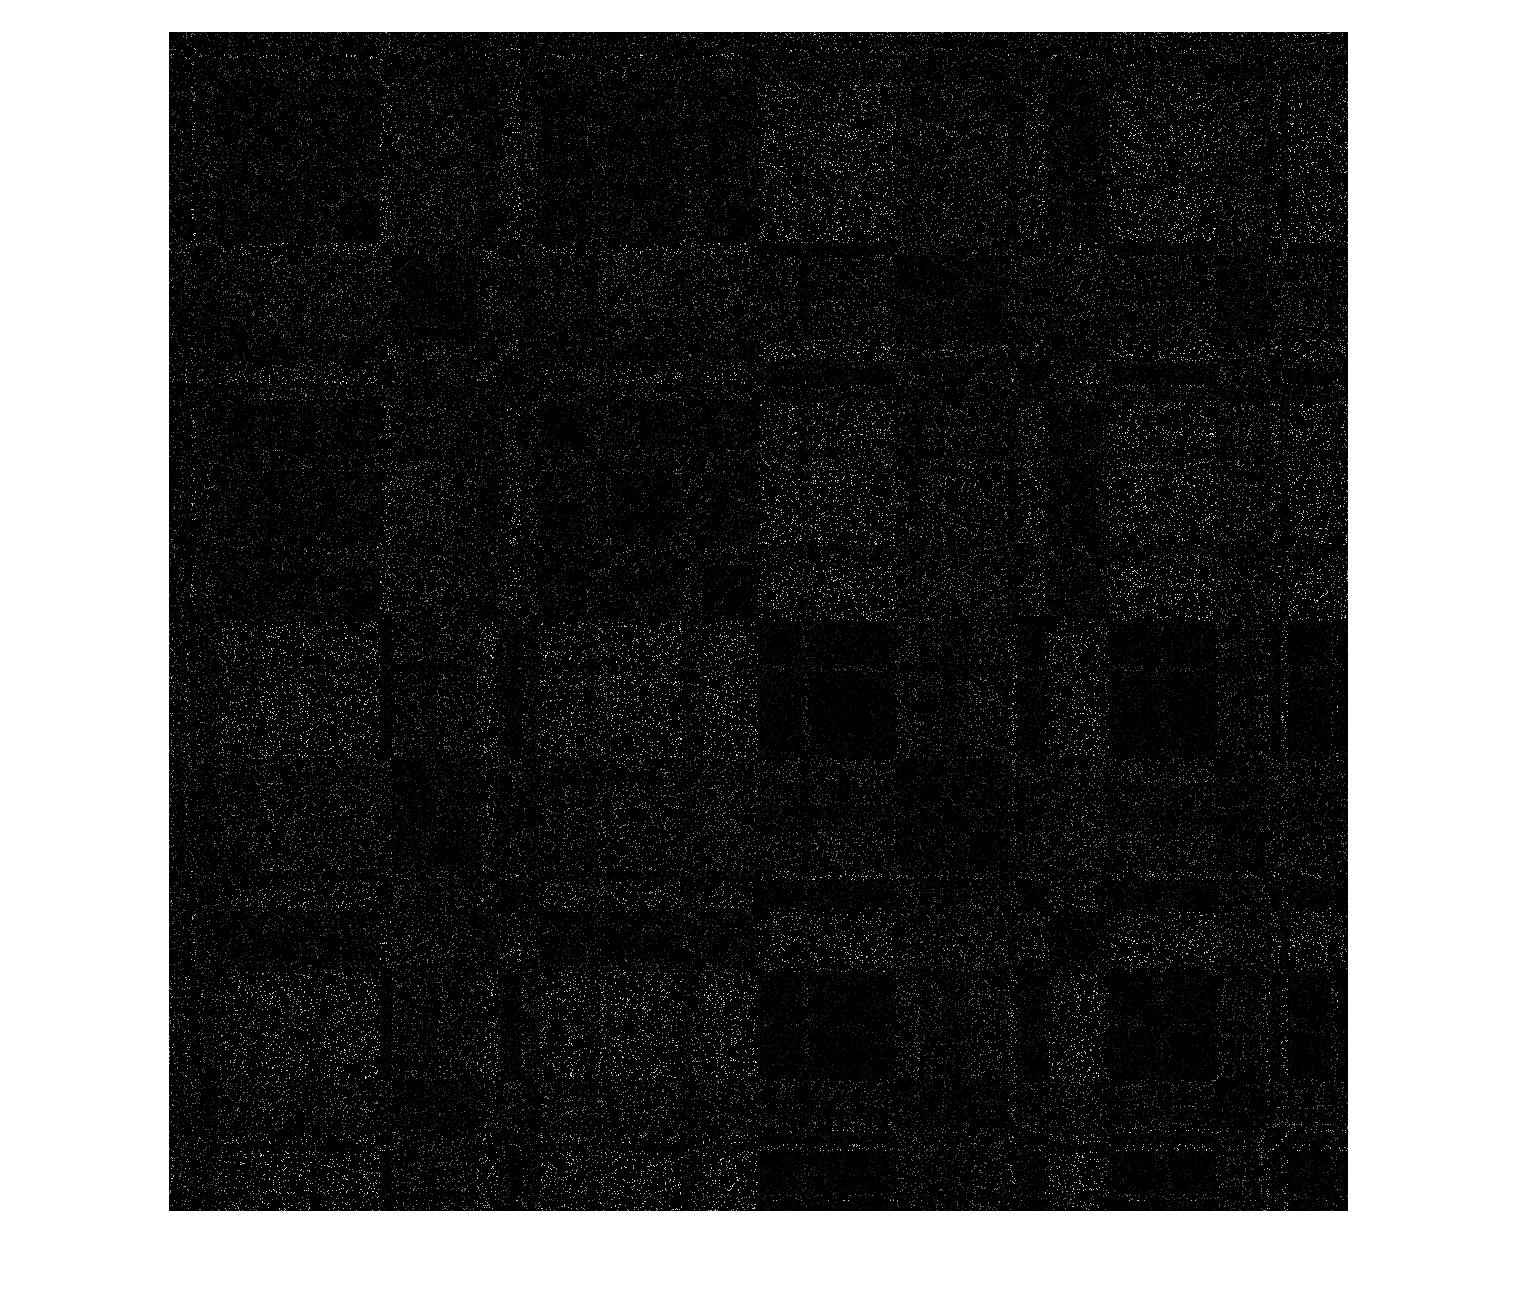
\includegraphics[width=1\linewidth]{before_dist.jpg}\\
\end{minipage}\hfill
\begin{minipage}{0.495\linewidth}
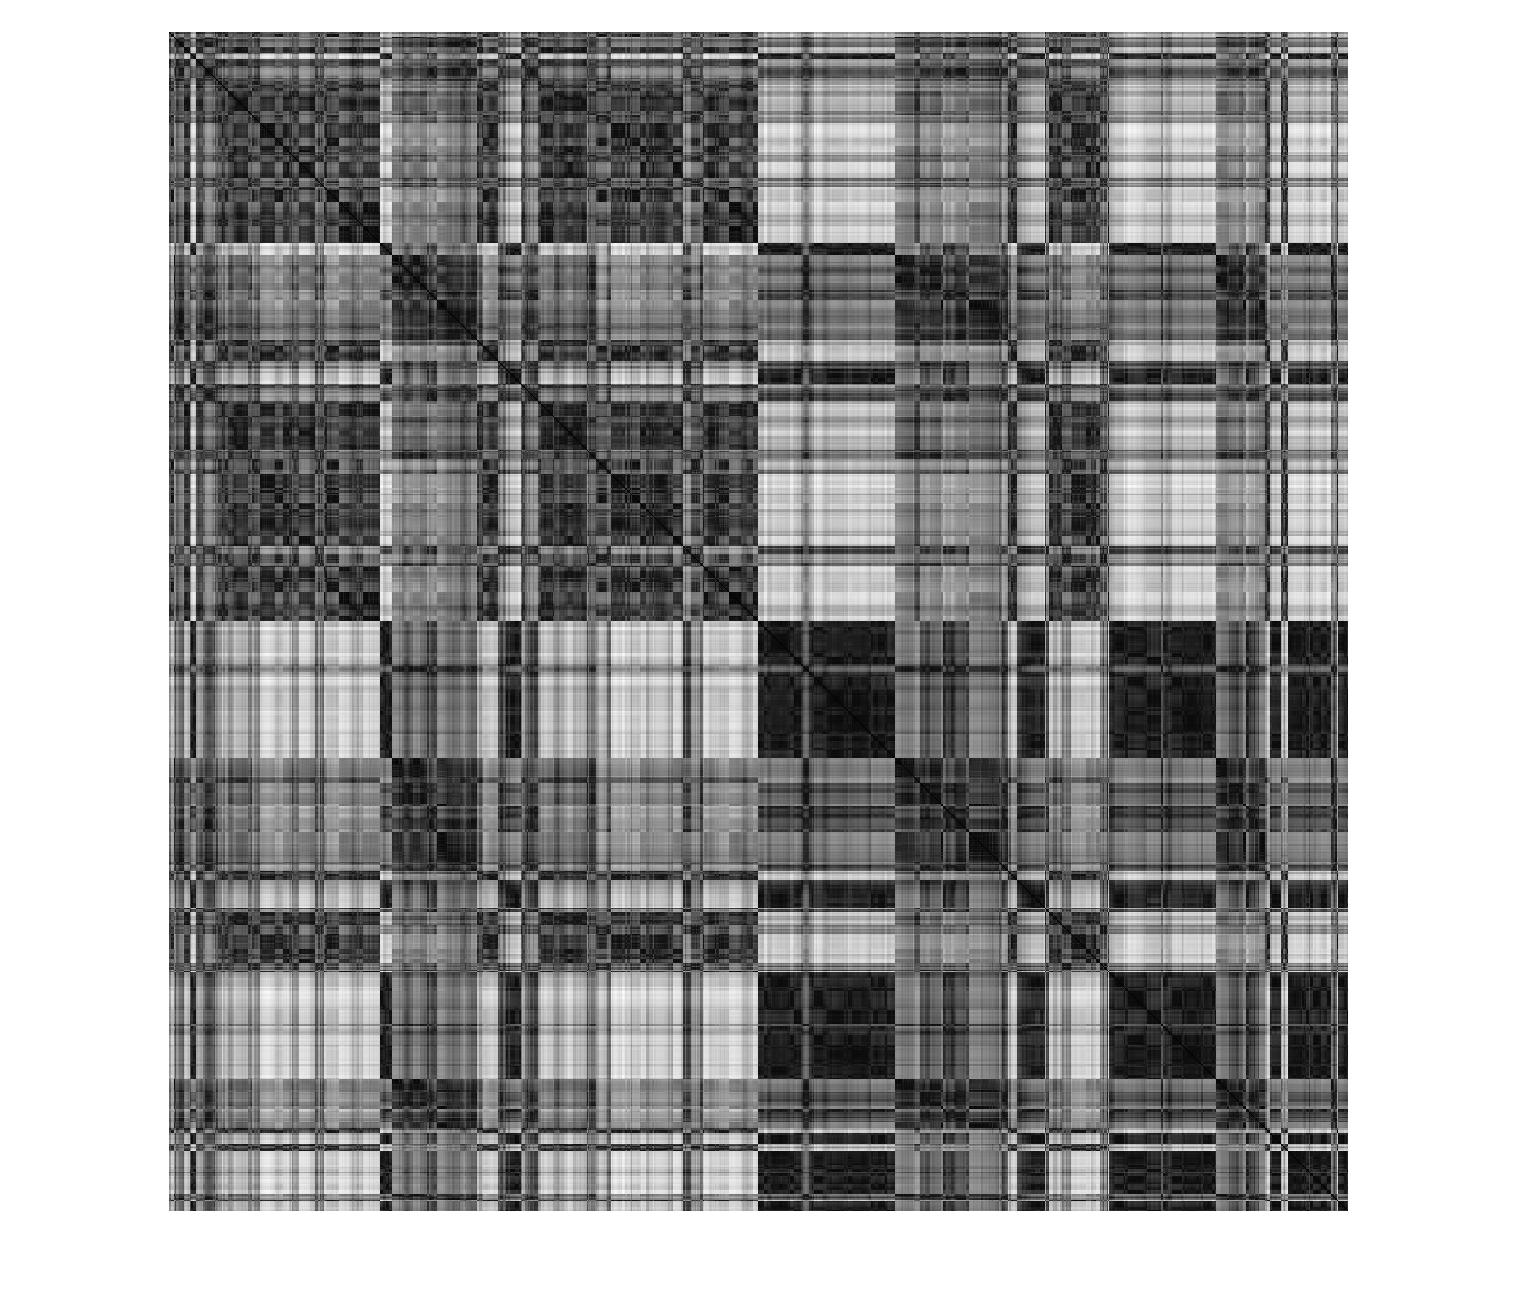
\includegraphics[width=1\linewidth]{after_dist.jpg}\\
\end{minipage}\hfill
\caption{Left: Available distance matrix. Right: Reconstructed distance matrix}
\end{figure}

\begin{figure}[H]
\centering
\begin{minipage}{0.495\linewidth}
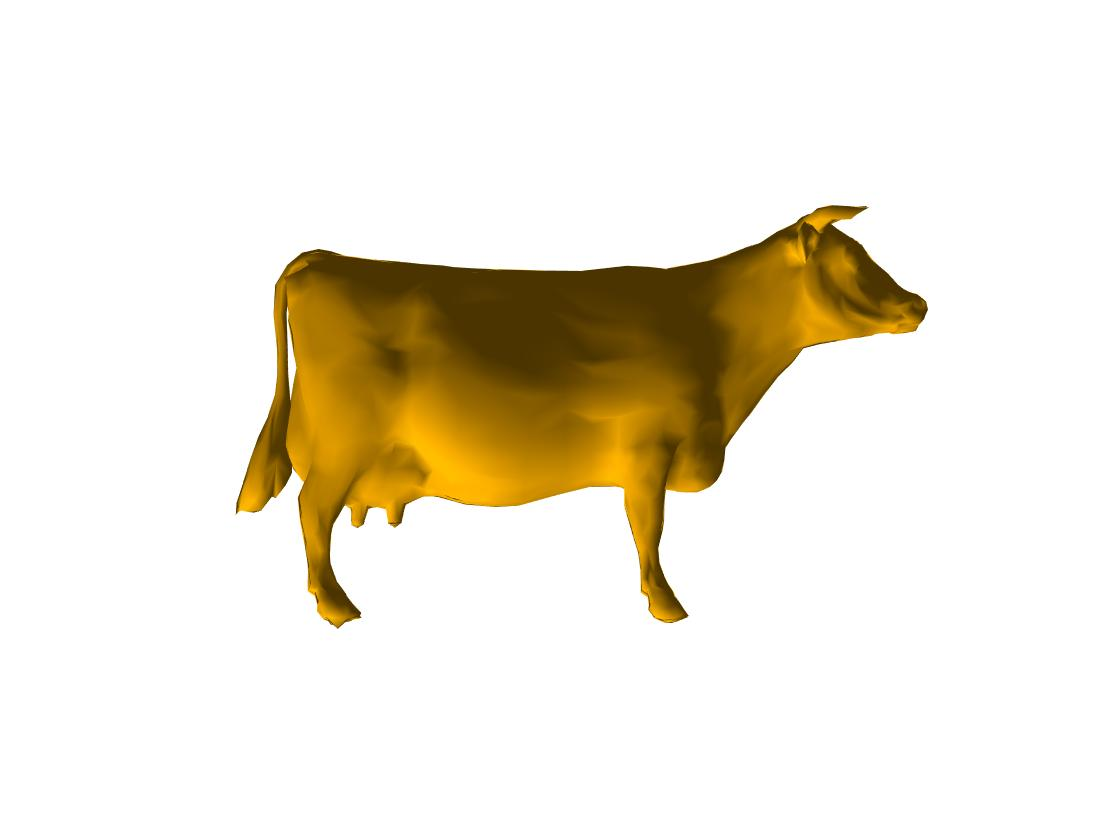
\includegraphics[width=1\linewidth]{cow1.jpg}\\
\end{minipage}\hfill
\begin{minipage}{0.495\linewidth}
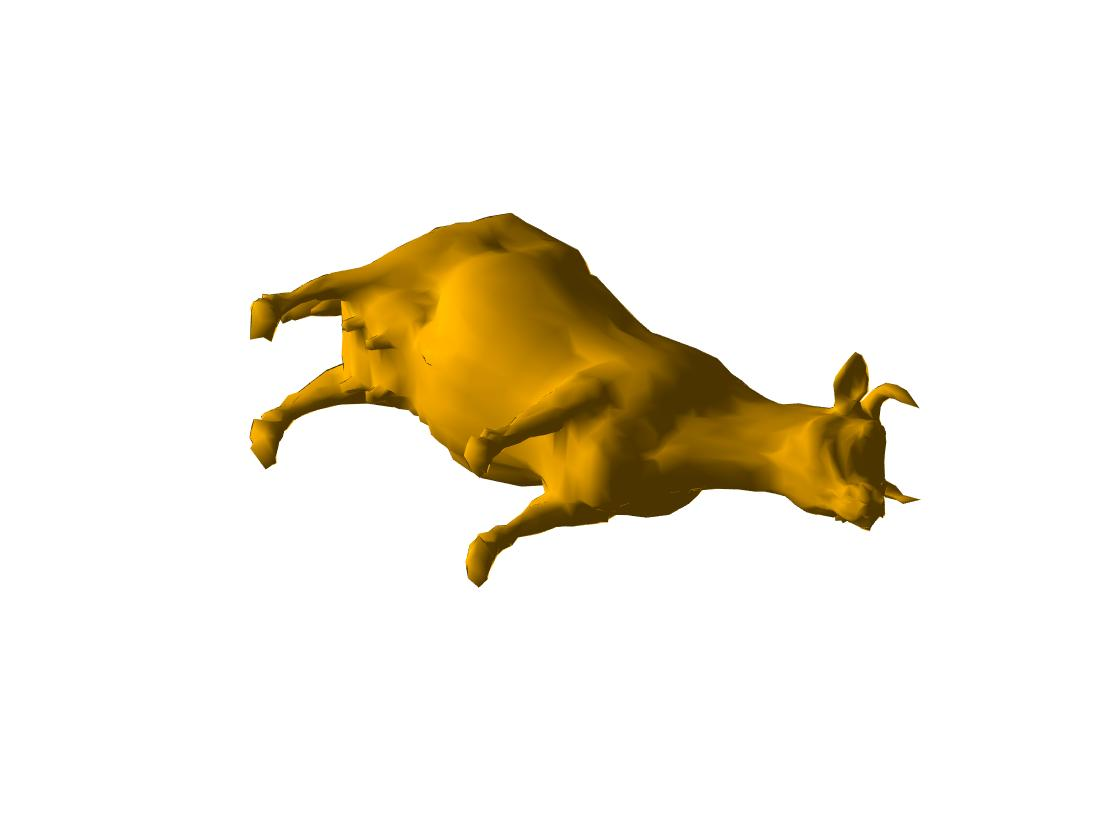
\includegraphics[width=1\linewidth]{cow2.jpg}\\
\end{minipage}\hfill
\caption{Two perspectives of reconstructed 3D cow}
\end{figure}


\section{Observation and Conclusions}

The recover result cow is relatively smooth. In this project we use singular value thresholding (SVT) algorithm to achieve data reconstruction based on incomplete inter-point distance problem. We successfully complete the matrix by using less than 4 percent of data from the whole matrix, and reconstructe the 3D cow. 
This paper introduce the singular value thresholding algorithm for matrix completion. This algorithm is easy to implement and surprisingly effective in terms of computational cost and storage requirement while the minimum nuclear-norm solution is also the lowest-rank solution.

\begin{thebibliography}{9}

\bibitem{cai2008}
Jian-Feng Cai, Emmanuel J. Cand\`{e}s and Zuowei Shen.
\textit{A Singular Value Thresholding Algorithm for Matrix Completion},
Singapore, 2008.

\end{thebibliography}


\bibliographystyle{unsrt}
\bibliography{projectreport}

\section*{Appendix}

\lstinputlisting{project.m}

\end{document}